\documentclass[a4paper,11pt]{article}
\usepackage[francais]{babel}
%\usepackage[french]{babel}
\usepackage{datetime} 

\usepackage{plantuml}
\usepackage{graphicx}

\usepackage[T1]{fontenc}
\usepackage{lmodern}

\usepackage[utf8]{inputenc}
\usepackage{xcolor}
\usepackage{listings}
\usepackage{enumitem}

\usepackage{listings}

\usepackage{plantuml}

% Profondeur de numérotation des sections
\setcounter{secnumdepth}{1}

\begin{document}

% Page de garde
\begin{titlepage}
    \centering
    \vspace*{\fill}
    {\Huge\textbf{Le `3 SPOT GAME' de Edward de Bono}} \\
    \vspace{20pt} % Ajoute un espace vertical de 10 points
    {\Large\textbf{R2.01- Developpement Oriente Objet}} \\
    \vspace{20pt} % Ajoute un espace vertical de 10 points
    {\textbf{M - Groupe } \\
    \vspace{20pt} % Ajoute un espace vertical de 10 points
    {\today} \\ % Date du jour
    \vspace*{\fill}}
\end{titlepage}

\tableofcontents

\newpage
\section{Introduction}
Ce rapport présente un programme informatique conçu pour deux joueurs ou s'affrontant au jeu de stratégie "3 Spot Game". Ce jeu de stratégie se joue sur un plateau de trois cases attribuant des points, où chaque joueur tente d'y placer sa pièce de couleur.

\subsection{1.1 Fonctionnalités du programme}

Le programme gère l'intégralité de la partie :
\begin{itemize}
    \item Affichage du plateau : Visualisation de l'état du plateau après chaque mouvement.
    \item Saisie des déplacements : Saisie des positions par les joueurs sur des emplacements disponibles et précalculés.
    \item Détection de la victoire : Détermination automatique du gagnant avec la règle spéciale qui spécifie que si un joueur termine la partie avec plus de 12 points, le second doit lui en avoir au moins 6.
    \item Gestion des points : Calcul des points gagnés par chaque joueur.
    \item Annonce du résultat : Informe les deux joueurs de qui a gagné.
\end{itemize}

\subsection{1.2 Gameplay interactif}

Le jeu est conçu pour une expérience interactive :
\begin{itemize}
    \item Alternance des joueurs : Chaque joueur place sa pièce à tour de rôle.
    \item Pièce blanche : Le programme gère la pièce blanche déplacée par chaque joueur à tour de rôle.
    \item Information du joueur : Affichage de la position actuelle du plateau, des options de déplacement disponibles avant chaque mouvement et du score.
\end{itemize}

Ce rapport détaille la conception du programme, son implémentation, ses fonctionnalités et les tests effectués pour garantir son bon fonctionnement.

\newpage
\section{Diagramme (UML) de dépendance}
\begin{center}
   
    \centering
    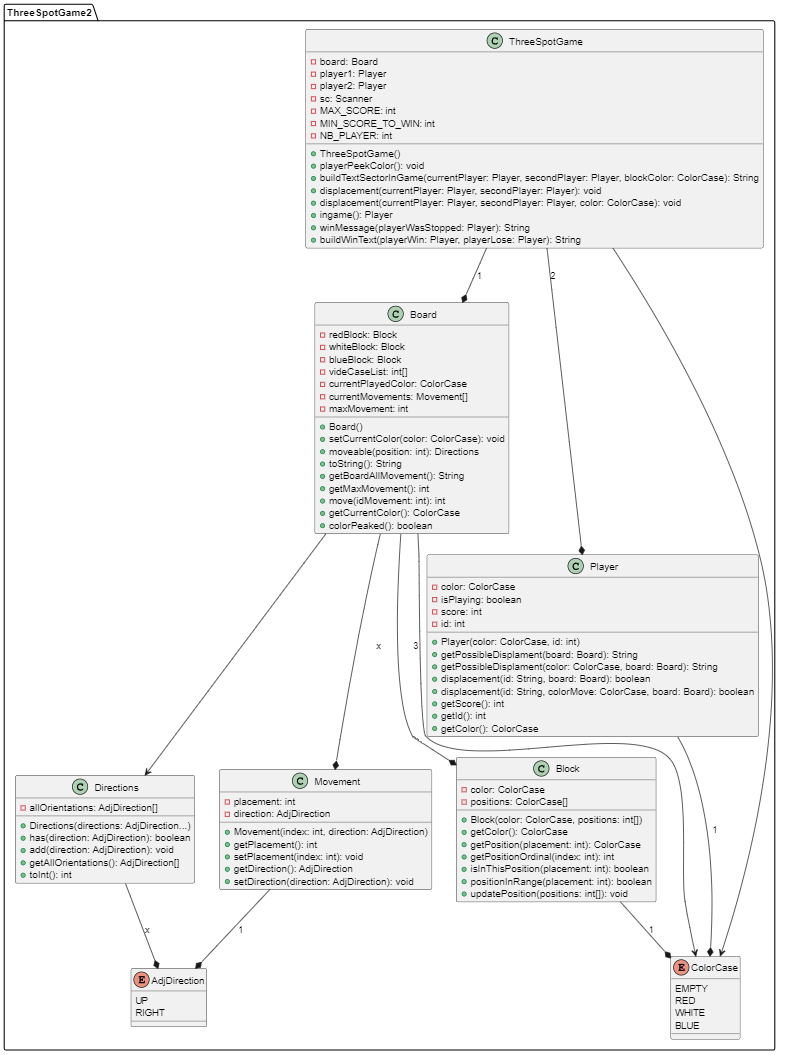
\includegraphics[scale=0.5]{diagrameUML.png}
    FIGURE 1 - Diagramme UML des classes formant l'application
\end{center}


\newpage
\section{Tests Unitaires}
\subsection{3.1 BlockTest.java (valide)}

\begin{lstlisting}[language=Java]
public class BlockTest {

    @Test
    public void testConstructor() {
        // Test constructor with valid positions
        int[] positions = {0, 1, 2};
        Block block = new Block(ColorCase.RED, positions);
        assertEquals(ColorCase.RED, block.getColor());
        assertEquals(ColorCase.RED, block.getPosition(0));
        assertEquals(ColorCase.RED, block.getPosition(1));
        assertEquals(ColorCase.RED, block.getPosition(2));
        assertNotEquals(ColorCase.RED, block.getPosition(3));

        // Test constructor with empty color
        assertThrows(AssertionError.class,
        () -> new Block(ColorCase.EMPTY, positions));
        
        // Test constructor with null color
        assertThrows(AssertionError.class,
        () -> new Block(null, positions));

        // Test constructor with null positions
        assertThrows(AssertionError.class,
        () -> new Block(ColorCase.RED, null));
        
    }

    @Test
    public void testPositionListNotToLongOrToShort() {
        // Test with valid positions
        int[] validP = {0, 1, 2};
        assertTrue(Block.positionListNotToLongOrToShort(validP));

        // Test with null positions
        int[] nullP = null;
        assertFalse(Block.positionListNotToLongOrToShort(nullP));

        // Test with empty positions a null block
        int[] emptyP = {};
        assertTrue(Block.positionListNotToLongOrToShort(emptyP));

        // Test with positions exceeding max size
        // Exceeds maximum size
        int[] exceedingSizePositions={0, 1, 2, 3, 4, 5, 6, 7, 8, 9}; 
        assertFalse(Block.positionListNotToLongOrToShort(
            exceedingSizePositions)
        );
    }


    @Test
    public void testGetPositionOutOfRange() {
        int[] positions = {0, 1, 2};
        Block block = new Block(ColorCase.RED, positions);
        // Lambda is mandatory to verify the assertions
        assertThrows(AssertionError.class,
        () -> block.getPosition(-1));
        
        assertThrows(AssertionError.class,
        () -> block.getPosition(Board.SIZE));
    }


    @Test
    public void testGetColor() {
        // Creating a block with a specific color and positions
        int[] positions = {0, 1, 2};
        Block block = new Block(ColorCase.RED, positions);
        
        // Verifying that the color is correct
        assertEquals(ColorCase.RED, block.getColor());

        // Verifying that the color of the block
        // is different from BLUE and WHITE
        assertNotEquals(ColorCase.BLUE, block.getColor());
        assertNotEquals(ColorCase.WHITE, block.getColor());
    }

    @Test
    public void testGetPosition() {
        // Creating a block with a specific color and positions
        int[] positions = {0, 1, 2};
        Block block = new Block(ColorCase.RED, positions);
        
        // Verifying that the color is correct
        //at the specified positions
        assertEquals(ColorCase.RED, block.getPosition(0));
        assertEquals(ColorCase.RED, block.getPosition(1));
        assertEquals(ColorCase.RED, block.getPosition(2));
        
        // Verifying positions out of range throw exceptions
        assertThrows(AssertionError.class,
        () -> block.getPosition(-1));
        
        assertThrows(AssertionError.class,
        () -> block.getPosition(Board.SIZE));
    }


    @Test
    public void testGetPositionOrdinal() {
        int[] positions = {0, 1, 2};
        Block block = new Block(ColorCase.RED, positions);
        assertEquals(ColorCase.RED.ordinal(), 
        block.getPositionOrdinal(0));
        
        assertEquals(ColorCase.RED.ordinal(),
        block.getPositionOrdinal(1));
        
        assertEquals(ColorCase.RED.ordinal(),
        block.getPositionOrdinal(2));
        
        assertNotEquals(ColorCase.RED.ordinal(),
        block.getPositionOrdinal(Board.SIZE-1));
        
        assertEquals(ColorCase.EMPTY.ordinal(),
        block.getPositionOrdinal(Board.SIZE-1));
    }

    @Test
    public void testIsInThisPosition() {
        int[] positions = {0, 1, 2};
        Block block = new Block(ColorCase.RED, positions);
        assertTrue(block.isInThisPosition(0));
        assertTrue(block.isInThisPosition(1));
        assertTrue(block.isInThisPosition(2));
        assertFalse(block.isInThisPosition(3));
    }

    @Test
    public void testUpdatePosition() {
        int[] positions = {0, 1, 2};
        Block block = new Block(ColorCase.RED, positions);
        block.updatePosition(3, 4, 5);
        assertEquals(ColorCase.RED, block.getPosition(3));
        assertEquals(ColorCase.RED, block.getPosition(4));
        assertEquals(ColorCase.RED, block.getPosition(5));
    }
}

\end{lstlisting}

\subsection{3.2 BoardTest.java (valide)}

\begin{lstlisting}[language=Java]
public class BoardTest {
    @Test
    public void testSetCurrentColor() {
        Board board = new Board();
        board.setCurrentColor(ColorCase.RED);
        assertEquals(ColorCase.RED, board.getCurrentColor());
    }

    @Test
    public void testGetCurrentColor() {
        Board board = new Board();
        assertNull(board.getCurrentColor());

        board.setCurrentColor(ColorCase.RED);
        assertEquals(ColorCase.RED, board.getCurrentColor());
    }

    @Test
    public void testColorPeaked() {
        Board board = new Board();
        assertFalse(board.colorPeaked());
        board.setCurrentColor(ColorCase.RED);
        assertTrue(board.colorPeaked());
    }

    @Test
    public void testMove() {
        Board board = new Board();
        String s = board.toString();
        board.setCurrentColor(ColorCase.RED);
        board.getBoardAllMovement();
        board.move(1);
        assertNotEquals(s, board.toString());

        assertEquals(board.toString(), 
        "* * * * * * * * * * * * *\n"
        +"*       *       *       *\n"
        +"*   R   *   R   *   O   *\n"
        +"*       *       *       *\n"
        +"* * * * * * * * * * * * *\n"
        +"*       *       *       *\n"
        +"*       *   W   *   W   *\n"
        +"*       *       *       *\n"
        +"* * * * * * * * * * * * *\n"
        +"*       *       *       *\n"
        +"*       *   B   *   B   *\n"
        +"*       *       *       *\n"
        +"* * * * * * * * * * * * *\n");
        
    }

    @Test
    public void testGetBoardAllMovement() {
        Board board = new Board();
        board.setCurrentColor(ColorCase.RED);
        //board must be tostringed one time before getBoardAllMovement
        board.toString();
        
        String boardString = board.getBoardAllMovement();
        assertEquals(boardString, "* * * * * * * * * * * * *\n" + 
                                  "*       *       *       *\n" + 
                                  "*   1   *       *   O   *\n" + 
                                  "*       *       *       *\n" + 
                                  "* * * * * * * * * * * * *\n" + 
                                  "*       *       *       *\n" + 
                                  "*   2   *   W   *   W   *\n" + 
                                  "*       *       *       *\n" + 
                                  "* * * * * * * * * * * * *\n" + 
                                  "*       *       *       *\n" + 
                                  "*   3   *   B   *   B   *\n" + 
                                  "*       *       *       *\n" + 
                                  "* * * * * * * * * * * * *\n" + 
                                  "");

        Board boardB = new Board();
        boardB.setCurrentColor(ColorCase.BLUE);
        //board must be tostringed one time before getBoardAllMovement
        boardB.toString();
        
        String boardStringB = boardB.getBoardAllMovement();
        assertEquals(boardStringB, "* * * * * * * * * * * * *\n" + 
                                  "*       *       *       *\n" + 
                                  "*       *   R   *   R   *\n" + 
                                  "*       *       *       *\n" + 
                                  "* * * * * * * * * * * * *\n" + 
                                  "*       *       *       *\n" + 
                                  "*   1   *   W   *   W   *\n" + 
                                  "*       *       *       *\n" + 
                                  "* * * * * * * * * * * * *\n" + 
                                  "*       *       *       *\n" + 
                                  "* 2 - 3 *       *   O   *\n" + 
                                  "*       *       *       *\n" + 
                                  "* * * * * * * * * * * * *\n" + 
                                  "");

    }
}


\end{lstlisting}
\newpage
\subsection{3.3 DirectionsTest.java (valide)}

\begin{lstlisting}[language=Java]
public class DirectionsTest {

    @Test
    public void testConstructorWithDirections() {
        // Test constructor with specified directions
        Directions directions1 =
            new Directions(AdjDirection.UP, AdjDirection.RIGHT);
        AdjDirection[] allO1 = directions1.getAllOrientations();

        // Verify that the specified directions are added correctly
        assertTrue(directions1.has(AdjDirection.UP));
        assertTrue(directions1.has(AdjDirection.RIGHT));

        // Verify that other orientations remain null
        for (AdjDirection direction : allO1) {
            if (direction != AdjDirection.UP 
            && direction != AdjDirection.RIGHT) {
                assertNull(direction);
            }
        }

        // Test constructor with null directions
        Directions directions2 = new Directions(null, null);
        AdjDirection[] allOrientations2 = 
            directions2.getAllOrientations();

        Directions directions3 = new Directions(null);
        AdjDirection[] allOrientations3 = 
            directions3.getAllOrientations();

        // Verify that all orientations are initialized to null
        for (AdjDirection direction : allOrientations2) {
            assertNull(direction);
        }

        for (AdjDirection direction : allOrientations3) {
            assertNull(direction);
        }


        Directions directions4 = new Directions(AdjDirection.UP);
        assertTrue(directions4.has(AdjDirection.UP));
        assertFalse(directions4.has(AdjDirection.RIGHT));


        Directions directions5 =
            new Directions(AdjDirection.UP, AdjDirection.UP);
        assertTrue(directions5.has(AdjDirection.UP));
        assertFalse(directions5.has(AdjDirection.RIGHT));

        Directions directions6 =
            new Directions(
                AdjDirection.RIGHT, 
                AdjDirection.RIGHT, 
                AdjDirection.UP, 
                djDirection.UP, 
                AdjDirection.RIGHT
            );
                
        assertTrue(directions6.has(AdjDirection.UP));
        assertTrue(directions6.has(AdjDirection.RIGHT));
    }

    @Test
    public void testHasMethod() {
        // Test has method with existing direction
        Directions directions1 = new Directions(AdjDirection.UP);
        assertTrue(directions1.has(AdjDirection.UP));

        // Test has method with non-existing direction
        Directions directions2 = new Directions();
        assertFalse(directions2.has(AdjDirection.RIGHT));

        // Test has method with null direction
        Directions directions3 = new Directions();
        assertThrows(AssertionError.class, () -> directions3.has(null));

        // Test has method with multiple directions
        Directions directions4 = 
            new Directions(AdjDirection.UP, AdjDirection.RIGHT);
        assertTrue(directions4.has(AdjDirection.UP));
        assertTrue(directions4.has(AdjDirection.RIGHT));
    }

    @Test
    public void testAddMethod() {
        // Test add method with existing direction
        Directions directions1 = new Directions(AdjDirection.UP);
        // Adding the same direction
        directions1.add(AdjDirection.UP); 
        // Should remain true
        assertTrue(directions1.has(AdjDirection.UP)); 

        // Test add method with non-existing direction
        Directions directions2 = new Directions();
        directions2.add(AdjDirection.RIGHT);
        // Should be added
        assertTrue(directions2.has(AdjDirection.RIGHT)); 

        // Test add method with null direction
        Directions directions3 = new Directions();
        // Adding null direction
        assertThrows(AssertionError.class, () -> directions3.add(null)); 
        // Should not be added
        assertThrows(AssertionError.class, () -> directions3.has(null)); 

        // Test add method with multiple directions
        Directions directions4 = new Directions();
        directions4.add(AdjDirection.UP);
        directions4.add(AdjDirection.RIGHT);
        // Should be added
        assertTrue(directions4.has(AdjDirection.UP)); 
        // Should be added
        assertTrue(directions4.has(AdjDirection.RIGHT)); 
    }

    @Test
    public void testToIntMethod() {
        // Test toInt method with no directions
        Directions directions1 = new Directions();
        assertEquals(0, directions1.toInt()); // Should return 0

        // Test toInt method with single direction
        Directions directions2 = new Directions(AdjDirection.UP);
        assertEquals(1, directions2.toInt()); // Should return 1

        // Test toInt method with multiple directions
        Directions directions3 = 
        new Directions(AdjDirection.UP, AdjDirection.RIGHT);
        
        assertEquals(2, directions3.toInt()); // Should return 2

        // Test toInt method with null direction
        Directions directions4 = new Directions(null);
        assertEquals(0, directions4.toInt()); // Should return 0
    }
}


\end{lstlisting}

\newpage
\subsection{3.4 MovementTest.java (valide)}

\begin{lstlisting}[language=Java]
public class MovementTest {

    @Test
    public void testConstructor() {
        // Test constructor with valid index and direction
        int index = 3;
        AdjDirection direction = AdjDirection.RIGHT;
        Movement movement = new Movement(index, direction);
        assertEquals(index, movement.getPlacement());
        assertEquals(direction, movement.getDirection());


        // Test default constructor
        Movement movement2 = new Movement();
        assertEquals(0, movement2.getPlacement());
        assertEquals(AdjDirection.UP, movement2.getDirection());

        // Test constructor with invalid index
        assertThrows(AssertionError.class,
        () -> new Movement(-1, AdjDirection.UP));
        
        assertThrows(AssertionError.class,
        () -> new Movement(Board.SIZE, AdjDirection.UP));

        // Test constructor with null direction
        assertThrows(AssertionError.class, () -> new Movement(3, null));
    }

    @Test
    public void testSetPlacement() {
        // Test setPlacement method
        Movement movement = new Movement();
        int index = 4;
        movement.setPlacement(index);
        assertEquals(index, movement.getPlacement());

        // Test setPlacement method with invalid index
        Movement movement2 = new Movement();
        assertThrows(AssertionError.class,
        () -> movement2.setPlacement(-1));
        
        assertThrows(AssertionError.class,
        () -> movement2.setPlacement(Board.SIZE));
    }

    @Test
    public void testSetDirection() {
        // Test setDirection method
        Movement movement = new Movement();
        AdjDirection direction = AdjDirection.RIGHT;
        movement.setDirection(direction);
        assertEquals(direction, movement.getDirection());

        // Test setDirection method with null direction
        Movement movement2 = new Movement();
        assertThrows(AssertionError.class,
        () -> movement2.setDirection(null));
    }
}


\end{lstlisting}


\newpage
\subsection{3.5 BlockTest.java (valide)}

\begin{lstlisting}[language=Java]
public class PlayerTest {
    @Test
    public void testConstructor() {

        // Test with valid color (RED) and ID
        assertDoesNotThrow(() -> new Player(ColorCase.RED, 1));

        // Test with valid color (BLUE) and ID
        assertDoesNotThrow(() -> new Player(ColorCase.BLUE, 2));

        // Test with invalid color (EMPTY)
        assertThrows(AssertionError.class, 
        () -> new Player(ColorCase.EMPTY, 1));

         // Test with invalid color (NULL)
         assertThrows(AssertionError.class, 
         () -> new Player(null, 1));

        // Test with invalid color (WHITE)
        assertThrows(AssertionError.class, 
        () -> new Player(ColorCase.WHITE, 1));

        // Test with invalid ID (less than 1)
        assertThrows(AssertionError.class, 
        () -> new Player(ColorCase.RED, 0));

        // Test with invalid ID (greater than 2)
        assertThrows(AssertionError.class, 
        () -> new Player(ColorCase.RED, 3));

        Player player = new Player(ColorCase.RED, 1);

        assertEquals(ColorCase.RED, player.getColor());
        assertEquals(0, player.getScore());
        assertEquals(1, player.getId());

        Player playerB = new Player(ColorCase.BLUE, 2);

        assertEquals(ColorCase.BLUE, playerB.getColor());
        assertEquals(0, playerB.getScore());
        assertEquals(2, playerB.getId());

    }

    @Test
    public void testGetPossibleDisplament() {
        Board board = new Board();
        Player player = new Player(ColorCase.RED, 1);
        player.getPossibleDisplament(board);

        // board need string befor a displacement
        board.toString();

        assertEquals(player.getPossibleDisplament(board),  
        "* * * * * * * * * * * * *\n" + 
        "*       *       *       *\n" + 
        "*   1   *       *   O   *\n" + 
        "*       *       *       *\n" + 
        "* * * * * * * * * * * * *\n" + 
        "*       *       *       *\n" + 
        "*   2   *   W   *   W   *\n" + 
        "*       *       *       *\n" + 
        "* * * * * * * * * * * * *\n" + 
        "*       *       *       *\n" + 
        "*   3   *   B   *   B   *\n" + 
        "*       *       *       *\n" + 
        "* * * * * * * * * * * * *\n" + 
        "");

        Player playerB = new Player(ColorCase.BLUE, 2);
        board = new Board();
        // board need string befor a displacement
        board.toString();
        playerB.getPossibleDisplament(board);
        
        assertEquals(playerB.getPossibleDisplament(board), 
        "* * * * * * * * * * * * *\n" + 
        "*       *       *       *\n" + 
        "*       *   R   *   R   *\n" + 
        "*       *       *       *\n" + 
        "* * * * * * * * * * * * *\n" + 
        "*       *       *       *\n" + 
        "*   1   *   W   *   W   *\n" + 
        "*       *       *       *\n" + 
        "* * * * * * * * * * * * *\n" + 
        "*       *       *       *\n" + 
        "* 2 - 3 *       *   O   *\n" + 
        "*       *       *       *\n" + 
        "* * * * * * * * * * * * *\n" + 
        "");
    }

    @Test
    public void testDisplacement() {
        Board board = new Board();
        board.toString();
        Player player = new Player(ColorCase.RED, 1);

        Board board1 = new Board();
        board1.setCurrentColor(ColorCase.RED);

        // board need string befor a displacement
        board1.toString();

        player.getPossibleDisplament(board1);
        // Assuming the first movement is valid
        assertTrue(player.displacement("1", board1));

        Board board2 = new Board();
        board2.setCurrentColor(ColorCase.RED);
        board2.toString();
        player.getPossibleDisplament(board2);
        // Assuming the second movement is invalid
        assertThrows(AssertionError.class, 
        () -> player.displacement("100", board2));
        
        boolean good;
        try {
            good = player.displacement("100", board2);
        } catch (AssertionError e) {
            good = false;
        }

        assertFalse(good);

        Board board3 = new Board();
        board3.setCurrentColor(ColorCase.RED);
        board3.toString();
        player.getPossibleDisplament(board3);
        // Assuming the second movement is valid
        assertTrue(player.displacement("2", board3));

        Board board4 = new Board();
        board4.setCurrentColor(ColorCase.RED);
        board4.toString();
        player.getPossibleDisplament(board4);
        // Assuming the thierd movement is valid
        assertTrue(player.displacement("3", board4));

        Player player2 = new Player(ColorCase.BLUE, 1);
        Board board5 = new Board();
        board5.setCurrentColor(ColorCase.RED);
        board5.toString();
        player2.getPossibleDisplament(board5);
        // Assuming the thierd movement is valid
        assertTrue(player2.displacement("3", board5));
    }
}


\end{lstlisting}

\newpage
\subsection{3.6 ThreeSpotGameTest.java (valide)}

\begin{lstlisting}[language=Java]
public class ThreeSpotGameTest 
{
    @Test
    public void test() {
        ThreeSpotGame game;

    }

}

\end{lstlisting}
\newpage

\section{Code Source}

\subsection{4.1 AdjDirection.java}

\begin{lstlisting}[language=Java]

package fr.septmg.ThreeSpotGame2;

/**
 * This enumeration represents possible adjacent directions.
 */
public enum AdjDirection {
    //NULL,
    
    /**
     * The direction upwards.
     */
    UP,

    /**
     * The direction to the right.
     */
    RIGHT,
    
    // BOTH,
}

\end{lstlisting}
\newpage

\subsection{4.2 ColorCase.java}

\begin{lstlisting}[language=Java]

package fr.septmg.ThreeSpotGame2;

/**
 * Enum representing the color cases in the ThreeSpot game.
 */
public enum ColorCase {
    /**
     * Represents an empty case.
     */
    EMPTY,

    /**
     * Represents a case filled with the color red.
     */
    RED,

    /**
     * Represents a case filled with the color white.
     */
    WHITE,

    /**
     * Represents a case filled with the color blue.
     */
    BLUE
}


\end{lstlisting}
\newpage

\subsection{4.3 Block.java}

\begin{lstlisting}[language=Java, breaklines=true]

package fr.septmg.ThreeSpotGame2;

/**
 * Represents a block in the ThreeSpot game.
 */
public class Block {
    private ColorCase color;
    private ColorCase[] positions;

    /**
     * Constructs a new Block with the specified color and positions.
     *
     * @param color The color of the block.
     * @param positions The positions of the block on the board.
     * @throws AssertionError If the color is null or empty, or if the positions list is too long or too short.
     */
    public Block(ColorCase color, int[] positions) {
        assert color != null && color != ColorCase.EMPTY;
        assert positionListNotToLongOrToShort(positions);
        this.color = color;
        makePosition(positions);
    }

    /**
     * Creates positions array for the block based on the given positions.
     *
     * @param position The positions of the block on the board.
     * @throws AssertionError If the positions is out of range.
     */
    private void makePosition(int[] position) {
        this.positions = new ColorCase[Board.SIZE];
        for (int i : position) {
            assert (i >= 0 && i < Board.SIZE);
            this.positions[i] = color;
        }
    }

    /**
     * Checks if the given positions list is not too long or too short.
     *
     * @param position The positions list to check.
     * @return True if the positions list is not too long or too short, false otherwise.
     */
    public static boolean positionListNotToLongOrToShort(int[] position) {
        return position != null && position.length < Board.SIZE;
    }

    /**
     * Gets the color of the block.
     *
     * @return The color of the block.
     */
    public ColorCase getColor() {
        return color;
    }

    /**
     * Gets the color at the specified position.
     *
     * @param placement The position to check.
     * @throws AssertionError If the placement is out of bounds.
     * @return The color at the specified position.
     */
    public ColorCase getPosition(int placement) {
        assert positionInRange(placement);
        return positions[placement] == null ? ColorCase.EMPTY : positions[placement];
    }

    /**
     * Gets the ordinal value of the color at the specified position.
     *
     * @param index The position index.
     * @return The ordinal value of the color at the specified position.
     */
    public int getPositionOrdinal(int index) {
        return getPosition(index).ordinal();
    }

    /**
     * Checks if the block is in the specified position.
     *
     * @param placement The position to check.
     * @throws AssertionError If the placement is out of bounds.
     * @return True if the block is in the specified position, false otherwise.
     */
    public boolean isInThisPosition(int placement) {
        assert positionInRange(placement);
        return getPosition(placement) == color;
    }

    /**
     * Checks if the given position is within the range of the positions array.
     *
     * @param placement The position to check.
     * @return True if the position is within the range, false otherwise.
     */
    public boolean positionInRange(int placement) {
        return (placement >= 0 && placement < positions.length);
    }

    /**
     * Updates the positions of the block.
     *
     * @param positions The new positions of the block on the board.
     * @throws AssertionError If the positions list is too long or too short.
     */
    public void updatePosition(int... positions) {
        assert positionListNotToLongOrToShort(positions);
        makePosition(positions);
    }

    // You may include JavaDoc for private methods if deemed necessary for clarity or future maintenance.
}


\end{lstlisting}
\newpage

\subsection{4.4 Movement.java}

\begin{lstlisting}[language=Java, breaklines=true]

package fr.septmg.ThreeSpotGame2;

/**
 * Represents a movement in the game.
 */
public class Movement {
    private int placement;
    private AdjDirection direction;

    /**
     * Constructs a new Movement object with the specified index and direction.
     *
     * @param index The index of the movement.
     * @param direction The direction of the movement.
     * @throws AssertionError If the index is out of bounds or if the direction is null.
     */
    public Movement(int index, AdjDirection direction) {
        assert index >= 0 && index < Board.SIZE;
        assert direction != null;

        this.placement = index;
        this.direction = direction;
    }

    /**
     * Constructs a new Movement object with default values.
     */
    public Movement() {
        this(0, AdjDirection.UP);
    }

    /**
     * Gets the index of the movement.
     *
     * @return The index of the movement.
     */
    public int getPlacement() {
        return placement;
    }

    /**
     * Sets the index of the movement.
     *
     * @param index The new index of the movement.
     * @throws AssertionError If the index is out of bounds.
     */
    public void setPlacement(int index) {
        assert index >= 0 && index < Board.SIZE;
        this.placement = index;
    }

    /**
     * Gets the direction of the movement.
     *
     * @return The direction of the movement.
     */
    public AdjDirection getDirection() {
        return direction;
    }

    /**
     * Sets the direction of the movement.
     *
     * @param direction The new direction of the movement.
     * @throws AssertionError If the direction is null.
     */
    public void setDirection(AdjDirection direction) {
        assert direction != null;
        this.direction = direction;
    }
}



\end{lstlisting}
\newpage

\subsection{4.5 Directions.java}

\begin{lstlisting}[language=Java, breaklines=true]

package fr.septmg.ThreeSpotGame2;

/**
 * Utility class to manage directions in a game.
 */
public class Directions {

    private AdjDirection allOrientations[];

    /**
     * Constructs a new Directions object with the specified directions.
     *
     * @param directions The directions to initialize the object with.
     */
    public Directions(AdjDirection... directions) {
        allOrientations = new AdjDirection[AdjDirection.values().length];

        if (directions != null) {
            if (directions.length > 0) {
                for (int i = 0; i < directions.length; ++i) {
                    if (directions[i] != null && !has(directions[i])) {
                        allOrientations[directions[i].ordinal()] = directions[i];
                    }
                }
            }
        }
    }

    /**
     * Checks if the specified direction is present in the object.
     *
     * @param direction The direction to check.
     * @throws AssertionError If the direction is null.
     * @return True if the direction is present, false otherwise.
     */
    public boolean has(AdjDirection direction) {
        assert direction != null;
        return allOrientations[direction.ordinal()] != null;
    }

    /**
     * Adds a direction to the object.
     *
     * @param direction The direction to add.
     */
    public void add(AdjDirection direction) {
        if (!has(direction)) {
            allOrientations[direction.ordinal()] = direction;
        }
    }

    /**
     * Gets all the directions stored in the object.
     *
     * @return An array containing all the directions.
     */
    public AdjDirection[] getAllOrientations() {
        return allOrientations;
    }

    /**
     * Converts the directions to an integer value representing the count of directions present.
     *
     * @return The integer representation of the count of directions.
     */
    public int toInt() {
        int result = 0;

        for (int i = 0; i < allOrientations.length; ++i) {
            if (allOrientations[i] != null) {
                result += (allOrientations[i] != null) ? 1 : 0;
            }
        }

        return result;
    }
}



\end{lstlisting}
\newpage


\subsection{4.6 Player.java}

\begin{lstlisting}[language=Java, breaklines=true]

package fr.septmg.ThreeSpotGame2;

/**
 * Represents a player in the game.
 */
public class Player {
    private ColorCase color;
    private boolean isPlaying;
    private int score;
    private int id;

    /**
     * Constructs a new Player object with the specified color and ID.
     *
     * @param color The color assigned to the player.
     * @param id The unique identifier for the player.
     * @throws AssertionError If the color is null, empty, or WHITE, or if the ID is not positive or exceeds the maximum number of players.
     */
    public Player(ColorCase color, int id) {
        assert color != null && color != ColorCase.EMPTY && color != ColorCase.WHITE : "Invalid color for player.";
        assert id > 0 : "Invalid player ID.";
        assert id <= ThreeSpotGame.NB_PLAYER : "Player ID exceeds maximum number of players.";
        this.color = color;
        this.isPlaying = false;
        this.score = 0;
        this.id = id;
    }

    /**
     * Retrieves the possible displacements for the player on the given board.
     *
     * @param board The game board to analyze for possible movements.
     * @return A string representing the possible displacements for the player on the board.
     */
    public String getPossibleDisplament(Board board) {
        return getPossibleDisplament(this.color, board);
    }

    /**
     * Retrieves the possible displacements for the specified color on the given board.
     *
     * @param color The color for which to calculate possible displacements.
     * @param board The game board to analyze for possible movements.
     * @return A string representing the possible displacements for the specified color on the board.
     * @throws AssertionError If the specified color is not the player's color or WHITE.
     */
    public String getPossibleDisplament(ColorCase color, Board board) {
        assert color == this.color || color == ColorCase.WHITE : "Invalid color for player.";

        board.setCurrentColor(color);
        isPlaying = true;
        return board.getBoardAllMovement();
    }

    /**
     * Performs a displacement action based on the provided movement ID and updates the board and player's score accordingly.
     *
     * @param id The ID of the movement to execute.
     * @param board The game board on which to perform the movement.
     * @return True if the displacement was successful, false otherwise.
     * @throws AssertionError If the player is not currently playing, if the specified color is not the player's color or WHITE,
     *                        or if the provided movement ID is invalid.
     */
    public boolean displacement(String id, Board board) {
        return displacement(id, color, board);
    }

    /**
     * Performs a displacement action based on the provided movement ID and color, and updates the board and player's score accordingly.
     *
     * @param id The ID of the movement to execute.
     * @param colorMove The color associated with the movement.
     * @param board The game board on which to perform the movement.
     * @return True if the displacement was successful, false otherwise.
     * @throws AssertionError If the player is not currently playing, if the specified color is not the player's color or WHITE,
     *                        or if the provided movement ID is invalid.
     */
    public boolean displacement(String id, ColorCase colorMove, Board board) {
        assert isPlaying : "Player is not currently playing.";
        assert color == colorMove || color == ColorCase.WHITE : "Invalid color for player.";
        int i = 0;

        try {
            i = Integer.parseInt(id);
        } catch (NumberFormatException e) {
            return false;
        }

        boolean validId = i <= board.getMaxMovement();
        assert validId : "Invalid movement ID.";

        if (!validId) {
            return false;
        }

        int temp = board.move(i);
        if (colorMove == color) {
            score += temp;
        }

        isPlaying = false;
        return true;
    }

    /**
     * Retrieves the player's current score.
     *
     * @return The player's current score.
     */
    public int getScore() {
        return score;
    }

    /**
     * Retrieves the player's ID.
     *
     * @return The player's ID.
     */
    public int getId() {
        return id;
    }

    /**
     * Retrieves the color associated with the player.
     *
     * @return The color associated with the player.
     */
    public ColorCase getColor() {
        return color;
    }
}


\end{lstlisting}
\newpage


\subsection{4.7 ThreeSpotGame.java}

\begin{lstlisting}[language=Java, breaklines=true]

package fr.septmg.ThreeSpotGame2;

import java.util.Scanner;

/**
 * Represents the Three Spot Game, a two-player game where players aim to score points by making strategic moves on a board.
 * The game ends when a player reaches the maximum score or when the other player fails to meet the minimum score requirement.
 */
public class ThreeSpotGame {
    private Board board;
    private Player player1, player2;
    private Scanner sc;

    /** The maximum score a player can achieve in the game. */
    final static int MAX_SCORE = 12;
    
    /** The minimum score required for a player to win the game. */
    final static int MIN_SCORE_TO_WIN = 6;
    
    /** The number of players in the game. */
    final static int NB_PLAYER = 2;
    
    /**
     * Constructs a new instance of the Three Spot Game and initializes the game components.
     * Players choose their colors, play the game, and the winner is determined.
     */
    public ThreeSpotGame() {
        board = new Board();
        playerPeekColor();
        System.out.println(winMessage(ingame()));
        sc.close();
    }

    /**
     * Prompts the players to choose their colors (red or blue).
     * Initializes player1 and player2 based on the chosen colors.
     */
    private void playerPeekColor() {
        String input = "";
        sc = new Scanner(System.in);

        do {
            System.out.println("Choose the color of your player (R or B): ");
            input = sc.nextLine();
        }
        while (!input.equals("R") && !input.equals("B"));

        if(input.equals("R")) {
            player1 = new Player(ColorCase.RED, 1);
            player2 = new Player(ColorCase.BLUE, 2);
        } else {
            player1 = new Player(ColorCase.BLUE, 1);
            player2 = new Player(ColorCase.RED, 2);
        }
    }

    /**
     * Builds the text indicating the current player's information and prompt for displacement.
     *
     * @param currentPlayer The current player.
     * @param secondPlayer The opponent player.
     * @param blockColor The color of the block involved in the displacement.
     * @return The constructed text.
     */
    private String buildTextSectorInGame(Player currenPlayer, Player secondPlayer, ColorCase blockColor) {
        return new StringBuilder("Player ")
                .append(currenPlayer.getId())
                .append(" (Your Score ")
                .append(Integer.toString(currenPlayer.getScore()))
                .append(" to ")
                .append(Integer.toString(secondPlayer.getScore()))
                .append(") choose a displacement : (block ")
                .append(blockColor.toString())
                .append(")")
                .toString();
    }
    /**
     * Initiates the displacement process for the current player.
     * This method automatically uses the color of the current player for the displacement.
     *
     * @param currentPlayer The current player initiating the displacement.
     * @param secondPlayer The opponent player.
     */
    private void displacement(Player currenPlayer, Player secondPlayer) {
        displacement(currenPlayer, secondPlayer, currenPlayer.getColor());
    }

    /**
     * Initiates the displacement process for the current player with the specified color.
     *
     * @param currentPlayer The current player initiating the displacement.
     * @param secondPlayer The opponent player.
     * @param color The color of the block involved in the displacement.
     */
    private void displacement(Player currenPlayer, Player secondPlayer, ColorCase color) {
        board.setCurrentColor(color);
        boolean good = false;

        System.out.println(board);

        System.out.println(currenPlayer.getPossibleDisplament(color, board));
        do {
            System.out.println(buildTextSectorInGame(currenPlayer, secondPlayer, color));

            good = currenPlayer.displacement(sc.nextLine(), color, board);
        }
        while (!good);
    }

    /**
     * Runs the main game loop until one of the players achieves the maximum score or the game ends.
     *
     * @return The player who reached the maximum score first or null if the game ends without a winner.
     */
    private Player ingame() {
        Player playerWasStopped = null;
        while (player2.getScore() < MAX_SCORE && playerWasStopped == null)
        {
            displacement(player1, player2);
            if(player1.getScore() < MAX_SCORE) {
                displacement(player1, player2, ColorCase.WHITE);

                displacement(player2, player1);
                if(player2.getScore() < MAX_SCORE) {
                    displacement(player2, player1, ColorCase.WHITE);
                }
                else
                    playerWasStopped = player2;
            }
            else
                playerWasStopped = player1;
        }

        return playerWasStopped;
    }

    /**
     * Generates the win message based on the player who stopped the game.
     *
     * @param playerWasStopped The player who reached the maximum score.
     * @return The win message.
     * @throws AssertionError if playerWasStopped is null.
     */
    private String winMessage(Player playerWasStopped) {
        assert playerWasStopped != null;

        Player secondPlayer = playerWasStopped == player1 ? player2 : player1;

        return secondPlayer.getScore() < MIN_SCORE_TO_WIN ? buildWinText(secondPlayer, playerWasStopped) : buildWinText(playerWasStopped, secondPlayer);
    }

    /**
     * Constructs the win message based on the winning and losing players.
     *
     * @param playerWin The player who won the game.
     * @param playerLose The player who lost the game.
     * @return The constructed win message.
     */
    private String buildWinText(Player playerWin, Player playerLose) {
        return new StringBuilder("Player ")
                    .append(playerWin.getId())
                    .append(" wins !")
                    .append("\nWith ")
                    .append(playerWin.getScore())
                    .append(" points at ")
                    .append(playerLose.getScore())
                    .append(" points.")
                    .append(playerWin.getScore() < playerLose.getScore() ? new StringBuilder(" Player ")
                    .append(playerLose.getId())
                   .append(" forgot the minimum score rule (the second player need a minimum above or equals to ")
                   .append(Integer.toString(MIN_SCORE_TO_WIN)).append(").") : "")
                   .toString();
    }
}


\end{lstlisting}
\newpage

\subsection{4.8 Board.java}

\begin{lstlisting}[language=Java, breaklines=true]

package fr.septmg.ThreeSpotGame2;

/**
 * Represents the game board for the ThreeSpot game.
 */
public class Board {
    private Block redBlock;
    private Block whiteBlock;
    private Block blueBlock;

    private int[] videCaseList;

    private ColorCase currentPlayedColor;
    private Movement[] currentMovements;
    private int maxMovement;

    /**
     * The size of a block on the board.
     */
    static final int BLOCK_SIZE = 2;

    /**
     * The total size of the board.
     */
    static final int SIZE = 9;

    /**
     * The number of columns on the board.
     */
    static final int X_SIZE = 3;

    /**
     * The number of rows on the board.
     */
    static final int Y_SIZE = 3;

    /**
     * The number of blocks on the board.
     */
    static final int NB_BLOCK = 3;

    private static final int CASE_STRING_SIZE = 7;

    /**
     * Constructs a new Board object with default configurations.
     */
    public Board() {
        int x_milieu = (X_SIZE-1)/2, y_milieu = (Y_SIZE-1)/2;
        int tempRed[] = new int[BLOCK_SIZE], tempWhite[] = new int[BLOCK_SIZE], tempBlue[] = new int[BLOCK_SIZE];

        for(int i = 0; i < BLOCK_SIZE; ++i) {
            tempRed[i] = i + x_milieu;
            tempWhite[i] = i + x_milieu + y_milieu * X_SIZE;
            tempBlue[i] = i + x_milieu + (Y_SIZE - 1) * X_SIZE;
        }
        this.redBlock = new Block(ColorCase.RED, tempRed);
        this.whiteBlock = new Block(ColorCase.WHITE, tempWhite);
        this.blueBlock = new Block(ColorCase.BLUE, tempBlue);

        videCaseList = new int[X_SIZE * Y_SIZE - BLOCK_SIZE * NB_BLOCK];
        currentMovements = new Movement[videCaseList.length * AdjDirection.values().length];
    }

    /**
     * Sets the current played color.
     *
     * @param color The color to set as the current played color.
     * @throws AssertionError If the color is empty.
     */
    public void setCurrentColor(ColorCase color) {
        assert color != ColorCase.EMPTY;
        this.currentPlayedColor = color;
    }

     /**
     * Gets the color case at the specified position on the board.
     *
     * @param position The position on the board to check.
     * @return The color case at the specified position.
     */
    private ColorCase getCase(int position) {
        if (redBlock.isInThisPosition(position)) {
            return ColorCase.RED;
        } else if (whiteBlock.isInThisPosition(position)) {
            return ColorCase.WHITE;
        } else if (blueBlock.isInThisPosition(position)) {
            return ColorCase.BLUE;
        } else {
            return ColorCase.EMPTY;
        }
    }

    // private int getCaseValue(int position) {
    //     return getCase(position).ordinal();
    // }

     /**
     * Determines the directions in which the current player can move from the specified position.
     *
     * @param position The position on the board to check for moveable directions.
     * @return A Directions object representing the moveable directions from the specified position.
     */
    public Directions moveable(int position) {
        Directions direction = new Directions();

        // up direction test
        if(position >= Y_SIZE) {
            ColorCase temp = getCase(position - Y_SIZE);

            if(temp == ColorCase.EMPTY) {
                direction.add(AdjDirection.UP);
            }
            else if (temp == currentPlayedColor && getCase(position) == ColorCase.EMPTY) {
                direction.add(AdjDirection.UP);
            }
        }
        
        // right direction test
        if(position % X_SIZE < X_SIZE && (position + 1) % Y_SIZE != 0) {
            ColorCase temp = getCase(position + 1);

            if(temp == ColorCase.EMPTY) {
                direction.add(AdjDirection.RIGHT);

            } else if(temp == currentPlayedColor && getCase(position) == ColorCase.EMPTY) {
                direction.add(AdjDirection.RIGHT);
            }
        }

        return direction;
    }

    /**
     * Returns a string representation of the board. Use Before getALlMovements !
     * 
     *
     * @return A string representing the current state of the board.
     */
    public String toString() {
        ColorCase currCase;
        int videCaseListIndex = 0;
        StringBuilder sb = new StringBuilder("* * * * * * * * * * * * *\n*       *       *       *\n");

        for (int i = 0; i < SIZE; ++i) {
            if(i % X_SIZE == 0 && i != 0) {
                sb.append("*\n*       *       *       *\n* * * * * * * * * * * * *\n*       *       *       *\n");
            }

            sb.append("*");
            currCase = getCase(i);

            if(currCase == ColorCase.EMPTY) {
                sb.append(i % Y_SIZE == X_SIZE - 1 ? "   O   " : "       ");
                videCaseList[videCaseListIndex++] = i;
            }
            else 
                sb.append("   ").append(currCase.toString().charAt(0)).append("   ");
        }
        return sb.append("*\n*       *       *       *\n* * * * * * * * * * * * *\n").toString();
    }


    /**
     * Generates a string representation of the board including all possible movements for the current player.
     * Each empty cell is annotated with a number representing a possible movement, and occupied cells are labeled
     * with the corresponding player color. Use After String the board !
     *
     * @return A string representing the current state of the board with all possible movements annotated.
     * @throws AssertionError If the list of empty cells is empty or if the current played color is null or empty.
     */
    public String getBoardAllMovement() {
        assert videCaseList.length > 0;
        assert currentPlayedColor != null && currentPlayedColor != ColorCase.EMPTY;
        
        ColorCase currCase;
        int videCaseListIndex = 0, accDirection = 0;

        StringBuilder sb = new StringBuilder("* * * * * * * * * * * * *\n*       *       *       *\n");

        for(int i = 0; i < SIZE; ++i) {
            if(i % X_SIZE == 0 && i != 0) {
                sb.append("*\n*       *       *       *\n* * * * * * * * * * * * *\n*       *       *       *\n");
            }
            sb.append("*");
            currCase = getCase(i);

            if(videCaseListIndex < videCaseList.length && i == videCaseList[videCaseListIndex] || currCase == currentPlayedColor) {
                Directions moveable = moveable(i);
                int moveableInt = moveable.toInt();
                StringBuilder sd = new StringBuilder();
                
                for(int j = 0; j < moveable.toInt(); ++j) {
                    if(j > 0) {
                        sd.append(" - ");
                    }

                    sd.append(++accDirection);
                    
                    AdjDirection[] allowedOrientations = moveable.getAllOrientations();
                    
                    while(allowedOrientations[j] == null && j < moveableInt) {
                        ++j;
                    }

                    currentMovements[accDirection - 1] = new Movement(i, allowedOrientations[j]);
                }
                if(currCase == ColorCase.EMPTY)
                    ++videCaseListIndex;

                if(moveableInt == 0)
                    sb.append(i % Y_SIZE == X_SIZE - 1 ? "   O   " : "       ");
                else{
                    for (int j = 0; j < (CASE_STRING_SIZE - sd.length())/2 + 1; ++j) {
                        sb.append(" ");
                        sd.append(" ");
                    }

                    sb.append(sd.toString());
                }
            }
            else {
                

                if(currCase == ColorCase.EMPTY || currCase == currentPlayedColor) {
                    sb.append(i % Y_SIZE == X_SIZE - 1 ? "   O   " : "       ");
                }
                else
                    sb.append("   ").append(currCase.toString().charAt(0)).append("   ");
            }

        }
        maxMovement = accDirection;
        return sb.append("*\n*       *       *       *\n* * * * * * * * * * * * *\n").toString();
    }

    /**
     * Retrieves the maximum number of movements available on the board.
     *
     * @return The maximum number of movements available.
     */
    public int getMaxMovement() {
        return maxMovement;
    }
    
    /**
     * Moves the current player's piece according to the specified movement ID and updates the board accordingly. Use After getAllMovement !
     *
     * @param idMovement The ID of the movement to execute.
     * @return The points gained from the movement.
     * @throws AssertionError If the movement ID is invalid, or if the current played color is null or empty.
     */
    public int move(int idMovement) {
        assert idMovement <= maxMovement && idMovement > 0;
        assert currentPlayedColor != null && currentPlayedColor != ColorCase.EMPTY;

        --idMovement;
        int point;
        switch (currentPlayedColor) {
            case RED:
                point = updateblock(redBlock, currentMovements[idMovement]);
                break;
            
            case WHITE:
                point = updateblock(whiteBlock, currentMovements[idMovement]);
                break;

            case BLUE:
                point = updateblock(blueBlock, currentMovements[idMovement]);
                break;
            
            default:
                throw new IllegalStateException("Unexpected value: " + currentPlayedColor);
        }

        currentPlayedColor = null;
        return point;
    }

    /**
     * Updates the specified block's position based on the given movement and returns the points gained.
     *
     * @param block The block to update.
     * @param movement The movement to execute.
     * @return The points gained from the movement.
     */
    private int updateblock(Block block, Movement movement) {
        int point = 0;
        int currentPlacement = movement.getPlacement();
        if(movement.getDirection() == AdjDirection.UP) {
            block.updatePosition(currentPlacement, currentPlacement - Y_SIZE);
            
            if(currentPlacement % Y_SIZE == X_SIZE-1)
                point = BLOCK_SIZE;
        }
        else if(movement.getDirection() == AdjDirection.RIGHT) {
            block.updatePosition(currentPlacement, ++currentPlacement);

            if(currentPlacement % Y_SIZE == X_SIZE-1)
                point = 1;
        }

        return point;
    }

    /**
     * Retrieves the current color being played.
     *
     * @return The current color being played, or null if no color is currently being played.
     */
    public ColorCase getCurrentColor() {
        return currentPlayedColor;
    }

    /**
     * Checks if a color has been selected for the current turn.
     *
     * @return True if a color has been selected, otherwise false.
     */
    public boolean colorPeaked() {
        return currentPlayedColor != null;
    }

}


\end{lstlisting}
\newpage

\section{Conclusion}

L'intérêt principal de ce projet pour moi réside dans l'opportunité de travailler dans un environnement de développement orienté objet. J'ai cherché à minimiser au maximum les boucles, même si cela peut sembler étrange de devoir afficher le plateau avant de calculer les déplacements disponibles. Cependant, cette approche a permis de réduire le nombre de boucles parcourant le plateau à seulement deux. Bien que cela puisse sembler peu utile étant donné que le plateau ne comporte que neuf cases, la conception du code reste flexible, permettant d'envisager un plateau beaucoup plus vaste avec un nombre considérable de cases et de pièces. Cette approche améliore significativement les performances du programme.\vspace{10pt} % Ajoute un espace vertical de 10 points

En explorant cette direction, nous avons rencontré des défis liés à la gestion des données redondantes et à l'optimisation de l'utilisation de la mémoire. Par exemple, lors de la conception de la classe Block, nous avons hésité à utiliser un tableau vide aux emplacements où se trouvent les blocs. Bien que cela puisse sembler gourmand en mémoire, nos recherches sur Internet ont suggéré que c'était peut-être le meilleur compromis en termes de mémoire et de performances par rapport à d'autres structures de données telles que les hashmaps ou les listes. L'approche principale du code consiste à éviter de sauvegarder une matrice du plateau ou une liste complète, mais plutôt à consulter chaque bloc pour vérifier s'ils se trouvent dans la case spécifiée. Cela permet de minimiser les données redondantes et d'optimiser les déplacements de blocs de manière efficace et rapide.\vspace{10pt} % Ajoute un espace vertical de 10 points

La principale difficulté rencontrée a été lors des tests unitaires, où nous avons réalisé que les méthodes privées sont difficilement testables. Par conséquent, la classe ThreeSpotGame n'a pas été correctement testée.\vspace{10pt} % Ajoute un espace vertical de 10 points

En ce qui concerne l'UML, nous avons rencontré des problèmes, notamment avec l'outil PlantUML. Bien qu'il offre une approche pratique pour créer des diagrammes UML avec du texte, il présente certaines limitations telles que l'impossibilité de dessiner des flèches en pointillé. De plus, pour les cas où le nombre d'instances passées en paramètre est indéterminé, nous avons utilisé "X" pour indiquer un nombre variable, ce qui ne permet pas une représentation précise dans le diagramme.

\end{document}